%%%%%%%%%%%%
%
% $Autor: Wings $
% $Datum: 2019-03-05 08:03:15Z $
% $Pfad: Sketch.tex $
% $Version: 4250 $
% !TeX spellcheck = en_GB/de_DE
% !TeX encoding = utf8
% !TeX root = manual 
% !TeX TXS-program:bibliography = txs:///biber
%
%%%%%%%%%%%%

\chapter{Skizze}

Technische Übersicht des Tischförderbands

\bigskip
\begin{figure}[h!]
	\begin{center}
\resizebox{0.21\textwidth}{!}{%
	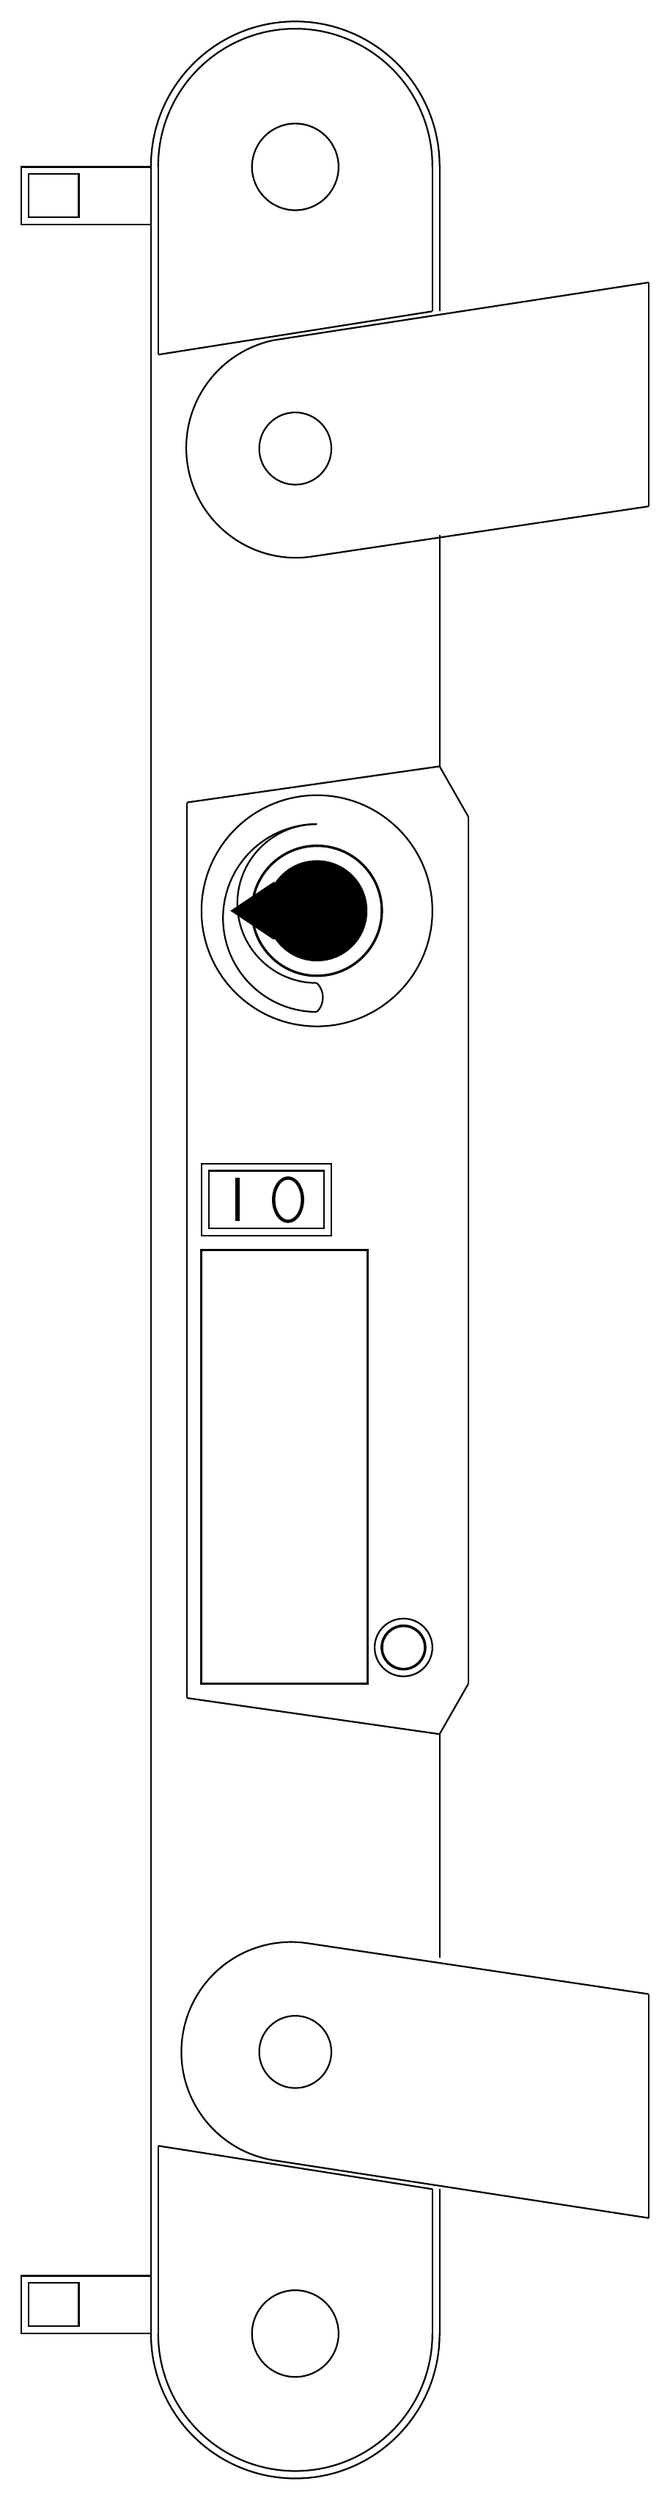
\begin{tikzpicture}[line width=0.8pt]
		
		\draw (20,-15.25) -- (20,22.25);
		\draw (25,22.25) -- (25,19.75);
		\draw (20,22.25) arc[start angle=-179.61, end angle=-360.39, radius=2.5001];
		\draw (25,-15.25) arc[start angle=0.15, end angle=-180.15, radius=2.5000];
		\draw (20.125,22.25) arc[start angle=-179.61, end angle=-360.39, radius=2.3751];
		\draw (24.875,22.25) -- (24.875,19.75);
		\draw (24.875,19.75) -- (20.125,19);
		\draw (20.125,19) -- (20.125,22.25);
		
		\draw (22.125,19.25) -- (28.625,20.25);
		\draw (28.625,20.25) -- (28.625,16.375);
		\draw (28.625,16.375) -- (22.75,15.5);
		\draw (22.75,15.5) arc[start angle=-82.86, end angle=-258.22, radius=1.9024];
		
		\draw (25,-15.25) -- (25,-12.75);
		\draw (24.875,-15.25) arc[start angle=0.08, end angle=-180.08, radius=2.3750];
		\draw (20.125,-15.25) -- (20.125,-12);
		\draw (24.875,-15.25) -- (24.875,-12.75);
		\draw (24.875,-12.75) -- (20.125,-12);
		
		\draw (22.125,-12.25) -- (28.625,-13.25);
		\draw (28.625,-13.25) -- (28.625,-9.375);
		\draw (28.625,-9.375) -- (22.75,-8.5);
		\draw (22.125,-12.25) arc[start angle=-99.16, end angle=-279.77, radius=1.9009];
		
		\draw (25,15.875) -- (25,11.875);
		\draw (25,11.875) -- (20.625,11.25);
		\draw (20.625,11.25) -- (20.625,-4.25);
		\draw (20.625,-4.25) -- (25,-4.875);
		\draw (25,-4.875) -- (25,-8.75);
		
		\draw (22.5,22.25) circle (0.75cm);
		\draw (22.5,-15.25) circle (0.75cm);
		\draw (22.5,17.375) circle (0.625cm);
		\draw (22.5,-10.375) circle (0.625cm);
		
		\draw (25,11.875) -- (25.5,11);
		\draw (25.5,11) -- (25.5,-4);
		\draw (25.5,-4) -- (25,-4.875);
		
		\draw[line width=1pt] (20.875,3.5) rectangle (23.75,-4);
		
		\draw (20,22.25) rectangle (17.75,21.25);
		\draw (20,-15.25) rectangle (17.75,-14.25);
		\draw (17.875,22.125) rectangle (18.75,21.375);
		\draw (17.875,-14.375) rectangle (18.75,-15.125);
		
		\draw (20.875,3.75) rectangle (23.125,5);
		\draw (21,3.875) rectangle (23,4.875);
		
		\draw[line width=2pt] (21.5,4.75) -- (21.5,4);
		\draw[line width=1.6pt] (22.375,4.375) ellipse (0.25cm and 0.375cm);
		
		\draw[line width=1.3pt] (24.375,-3.375) circle (0.375cm);
		\draw (24.375,-3.375) circle (0.5cm);
		
		\draw[line width=1.2pt] (22.875,9.375) circle (1.125cm);
		\draw[line width=0.8pt] (22.875,9.375) circle (2cm);
		
		\draw[line width=0.8pt] (22.875,8.125)
		arc[start angle=-89.85, end angle=-270.15, radius=1.3750];
		
		\draw[line width=0.8pt] (22.875,7.625)
		arc[start angle=-89.93, end angle=-270.07, radius=1.6250];
		
		\draw[line width=0.8pt] (22.875,8.125)
		arc[start angle=45.00, end angle=-45.00, radius=0.3536];
		
		\fill (22.875,9.375) circle (0.875cm);
		\fill (21.375,9.375) -- (22.125,8.875) -- (22.875,9.375) -- (22.125,9.875) -- cycle;
		
	\end{tikzpicture}
}
	\caption{Skizze mit echten Halbkreis-Rundungen}
	\end{center}
\end{figure}
%\begin{figure}
%	\begin{center}
%		\begin{tikzpicture}
			% Grundgerüst Förderband
%			\draw (-6,1) -- (6,1);
%			\draw (6,1) .. controls (6.5523, 1) and (7, 0.5523) .. (7,0)
%			.. controls (7, -0.5523) and (6.5523, -1) .. (6,-1); 
			% Werte in control mit Bezier-Kurven ermittelt
%			\draw (6,-1) -- (-6,-1);
%			\draw (-6,-1) .. controls (-6.5523,-1) and (-7,-0.5523) .. (-7,0)
%			.. controls (-7,0.5523) and (-6.5523,1) .. (-6,1);
			% Bedienerpult
%			\draw (0,-0.9) rectangle (3.7,0.7);
			% Display
%			\draw (0.1,-0.2) rectangle (2,0.6);
			 
			% An/Aus-Schalter
%			\draw (0.1,-0.3) rectangle (0.7,-0.7);
%			\draw (0.15,-0.35) rectangle (0.65,-0.65);
%			\draw (0.25,-0.4) -- (0.25,-0.6);
%			\draw (0.5,-0.5) ellipse [x radius=1.5pt, y radius=3pt];
			
		% Richtungsumkehr-Schalter	
		%	\draw (2.7,0) rectangle (3.1,0.5);
		%	\draw (2.8,0.1) rectangle (3.0,0.4);
			
		%Lichtschranken
			% rechts
%			\draw (4,1) -- (4,2);
%			\draw (4.7,1) -- (4.7,2);
%			\draw (4,2) -- (4.7,2);
%			\draw (4.1,1.3) rectangle (4.6,1.9);
			% links
%			\draw (-4,1) -- (-4,2);
%			\draw (-4.7,1) -- (-4.7,2);
%			\draw (-4,2) -- (-4.7,2);
%			\draw (-4.1,1.3) rectangle (-4.6,1.9);
		
		% Poti
%			\draw (2.5,0) circle [radius=0.3cm];
%			\draw (2.5,0) circle [radius=0.15cm];
%			\draw (2.5,0.2) -- (2.5,0.3);
		
			
		% Geraden rechter Stützfuß
%			\draw (4,-0.2) -- (4.3,-2.5);
			% linke Gerade
%			\draw (4.3,-2.5) -- (5.5,-2.5);
			% untere Gerade
%			\draw (5.5,-2.5) -- (5.2,-0.2);
			% rechte Gerade
%			\draw (4,-0.2) -- (5.2,-0.2);
			
			% Geraden linker Stützfuß
%			\draw (-4,-0.2) -- (-4.3,-2.5); 
			% linke Gerade (gespiegelt)
%			\draw (-4.3,-2.5) -- (-5.5,-2.5);
			% untere Gerade (gespiegelt)
%			\draw (-5.5,-2.5) -- (-5.2,-0.2);
			% rechte Gerade (gespiegelt)
%			\draw (-4,-0.2) -- (-5.2,-0.2);
		%Stützfüße
%		\end{tikzpicture}
%	\end{center}
%\end{figure}
